\section{Progress}

Where are we with design/implementation?

Full implementation of the Python Script that connects to the TomTom API and utilization of the Command Line interface to obtain image of a particular Longitude and Latitude with zoom and image style.

\begin{figure}[!ht]
    \centering
    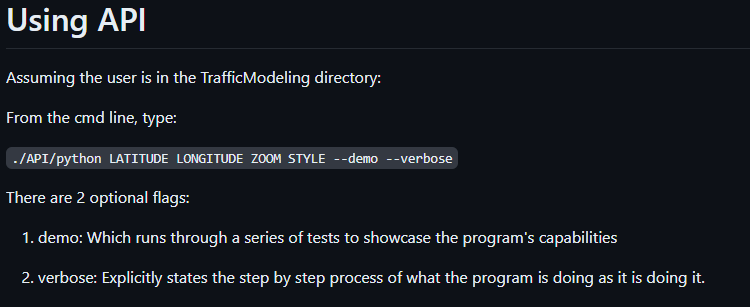
\includegraphics[width=10cm]{../Images/Update4/APIInstructions.png}
       \caption{How to use the Python Script.}
           \label{Fig:ConversionFunction}
\end{figure}

\begin{figure}[!ht]
    \centering
    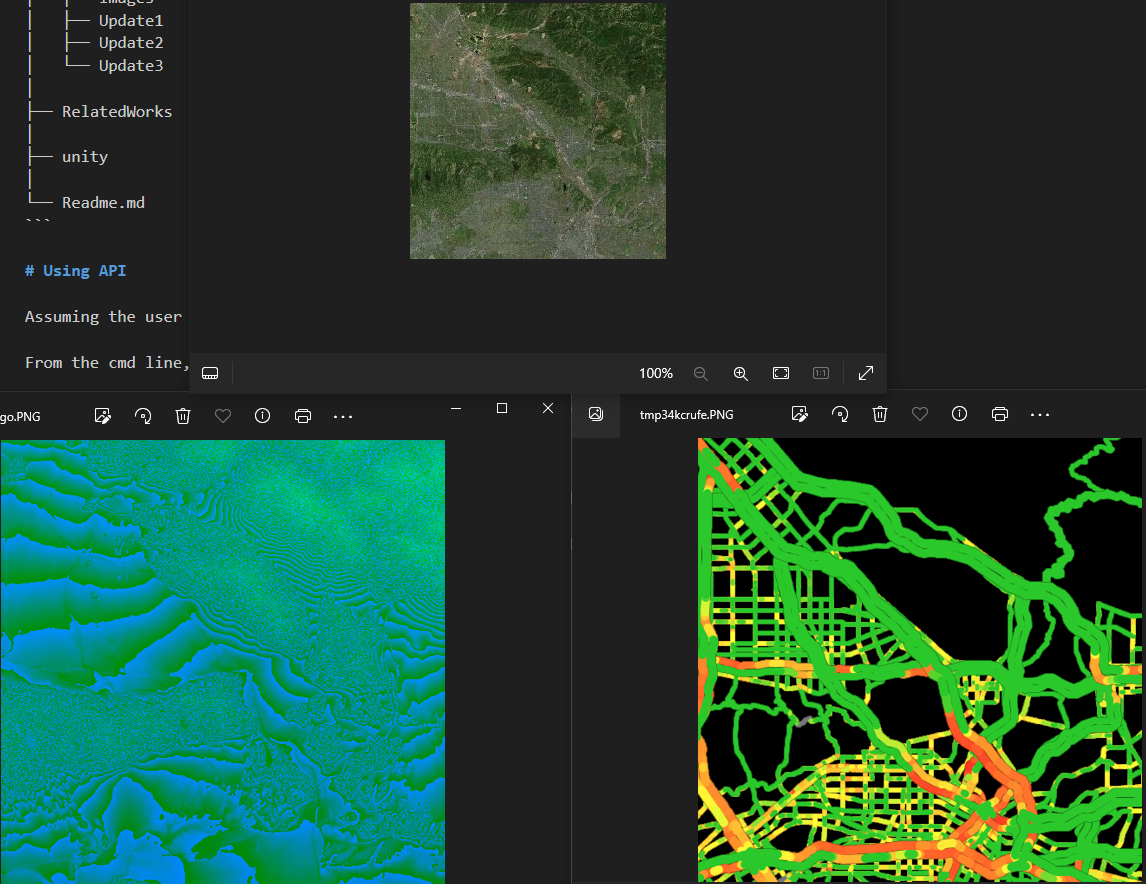
\includegraphics[width=10cm]{../Images/Update4/DemoAPI.png}
       \caption{Demo from script.}
           \label{Fig:ConversionFunction}
\end{figure}

\begin{flushleft}
Starting to think about the UI/UX of the program a little more and changed the camera position to follow the car moving from a distance. We also baked a new pathfinding scene from a new network of roads and traffic that include intersections and more streets.
\end{flushleft}

\begin{figure}[!ht]
    \centering
    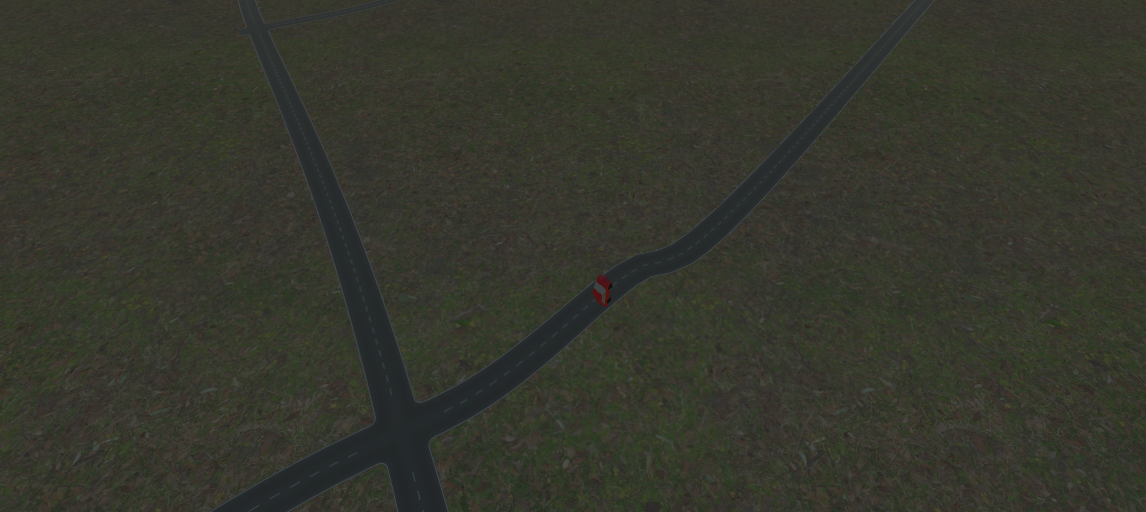
\includegraphics[width=10cm]{../Images/Update4/GameView.png}
       \caption{Camera view of scene from game screen.}
           \label{Fig:Gameview}
\end{figure}

\begin{flushleft}
With that, we started testing Unity's built in pathfinding function and seeing what limitations it has. A limitation we found was that between two roads, the pathfinding would have a preference for the road that it was closest to. If it was already on the road, it would continue further down. The issue here is that if there is an obstacle at the end of the road, then the object would continue down the path then be stuck when it ran into it. We would need to have a system that it could "see down the road" and choose to go the other way or it would continue down a road then turn around when it runs into an obstacle.
\end{flushleft}